\documentclass[12pt, border=10pt]{standalone}
\usepackage{tikz}
\usepackage{amsmath}
\usepackage{amssymb}
\usepackage{mathrsfs}

\begin{document}
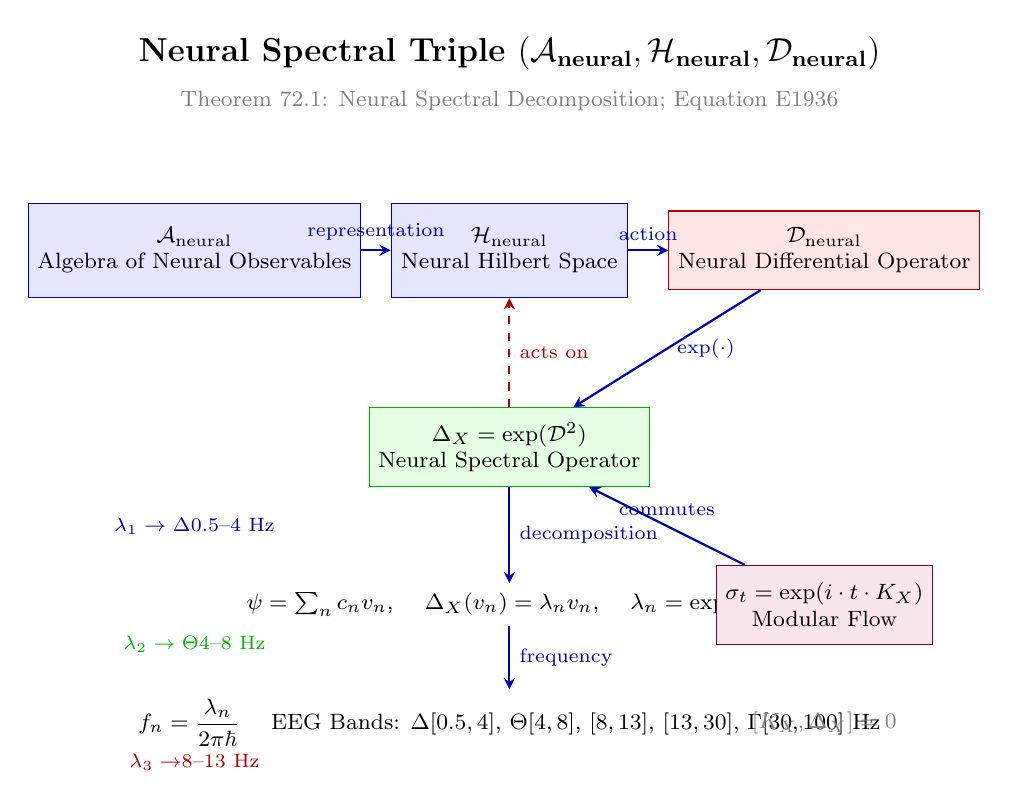
\begin{tikzpicture}[
    node distance=2.5cm,
    every node/.style={font=\small},
    spectral/.style={rectangle, draw=blue!70!black, fill=blue!10, minimum width=3cm, minimum height=1.2cm, align=center, font=\footnotesize},
    operator/.style={rectangle, draw=red!70!black, fill=red!10, minimum width=2.5cm, minimum height=1cm, align=center, font=\footnotesize},
    arrow/.style={->, >=stealth, thick, blue!70!black},
    dashed-arrow/.style={->, >=stealth, thick, red!70!black, dashed},
]

% Title
\node[font=\bfseries\large, text centered] at (0, 5) {Neural Spectral Triple $(\mathcal{A}_{\text{neural}}, \mathcal{H}_{\text{neural}}, \mathcal{D}_{\text{neural}})$};
\node[font=\footnotesize, text centered, text=gray] at (0, 4.4) {Theorem 72.1: Neural Spectral Decomposition; Equation E1936};

% Algebra A_neural
\node[spectral] (A) at (-4, 2.5) {$\mathcal{A}_{\text{neural}}$\\Algebra of Neural Observables};

% Hilbert Space H_neural
\node[spectral] (H) at (0, 2.5) {$\mathcal{H}_{\text{neural}}$\\Neural Hilbert Space};

% Differential Operator D_neural
\node[operator] (D) at (4, 2.5) {$\mathcal{D}_{\text{neural}}$\\Neural Differential Operator};

% Delta_X operator
\node[operator, draw=green!70!black, fill=green!10] (Delta) at (0, 0) {$\Delta_X = \exp(\mathcal{D}^2)$\\Neural Spectral Operator};

% Eigenvalue decomposition
\node[font=\footnotesize, text centered, text=black] (eigen) at (0, -2) {
    $\psi = \sum_n c_n v_n$, \quad $\Delta_X(v_n) = \lambda_n v_n$, \quad $\lambda_n = \exp(\mu_n)$
};

% Frequency mapping
\node[font=\footnotesize, text centered, text=black] (freq) at (0, -3.5) {
    $f_n = \dfrac{\lambda_n}{2\pi\hbar}$ \quad EEG Bands: $\Delta[0.5,4]$, $\Theta[4,8]$, $\Alpha[8,13]$, $\Beta[13,30]$, $\Gamma[30,100]$ Hz
};

% Modular flow
\node[operator, draw=purple!70!black, fill=purple!10] (sigma) at (4, -2) {$\sigma_t = \exp(i \cdot t \cdot K_X)$\\Modular Flow};

% Commutation relation
\node[font=\footnotesize, text centered, text=gray] (comm) at (4, -3.5) {$[K_X, \Delta_X] = 0$};

% Arrows connecting components
\draw[arrow] (A) -- (H) node[midway, above, font=\scriptsize] {representation};
\draw[arrow] (H) -- (D) node[midway, above, font=\scriptsize] {action};
\draw[arrow] (D) -- (Delta) node[midway, right, font=\scriptsize] {$\exp(\cdot)$};
\draw[dashed-arrow] (Delta) -- (H) node[midway, right, font=\scriptsize] {acts on};
\draw[arrow] (Delta) -- (eigen) node[midway, right, font=\scriptsize] {decomposition};
\draw[arrow] (eigen) -- (freq) node[midway, right, font=\scriptsize] {frequency};
\draw[arrow] (sigma) -- (Delta) node[midway, above, font=\scriptsize] {commutes};

% EEG band annotations
\node[font=\scriptsize, text=blue!70!black, text centered] at (-4, -1) {
    $\lambda_1 \to \Delta$\\0.5--4 Hz
};
\node[font=\scriptsize, text=green!70!black, text centered] at (-4, -2.5) {
    $\lambda_2 \to \Theta$\\4--8 Hz
};
\node[font=\scriptsize, text=red!70!black, text centered] at (-4, -4) {
    $\lambda_3 \to \Alpha$\\8--13 Hz
};

\end{tikzpicture}
\end{document}
